

\tikzset{every picture/.style={line width=0.75pt}} %set default line width to 0.75pt        

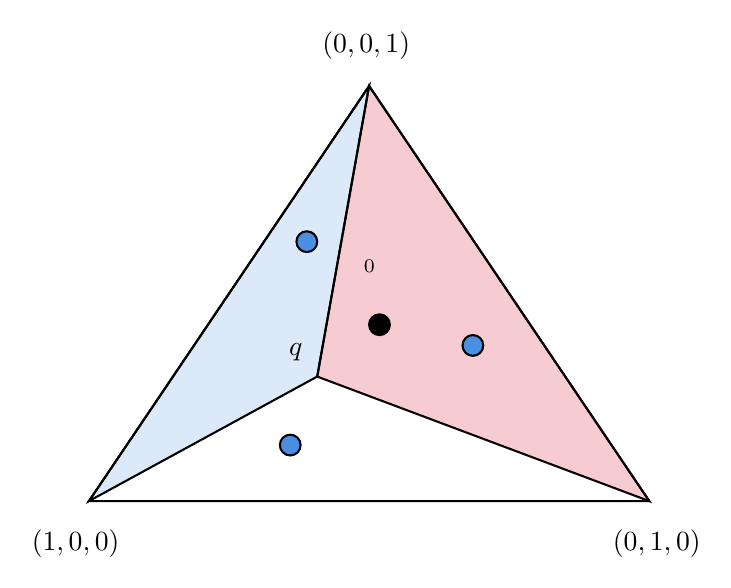
\begin{tikzpicture}[x=0.75pt,y=0.75pt,yscale=-1,xscale=1]
%uncomment if require: \path (0,300); %set diagram left start at 0, and has height of 300

%Shape: Polygon [id:ds12997950611396247] 
\draw  [fill={rgb, 255:red, 74; green, 144; blue, 226 }  ,fill opacity=0.2 ] (235,50) -- (210,190) -- (100,250) -- cycle ;
%Shape: Triangle [id:dp2663618049578823] 
\draw   (235,50) -- (370,250) -- (100,250) -- cycle ;
%Shape: Polygon [id:ds41194641592346326] 
\draw  [fill={rgb, 255:red, 208; green, 2; blue, 27 }  ,fill opacity=0.2 ] (235,50) -- (370,250) -- (210,190) -- cycle ;
%Shape: Circle [id:dp6296340315249684] 
\draw  [fill={rgb, 255:red, 0; green, 0; blue, 0 }  ,fill opacity=1 ] (235,165) .. controls (235,162.24) and (237.24,160) .. (240,160) .. controls (242.76,160) and (245,162.24) .. (245,165) .. controls (245,167.76) and (242.76,170) .. (240,170) .. controls (237.24,170) and (235,167.76) .. (235,165) -- cycle ;
%Shape: Circle [id:dp5483903323436823] 
\draw  [fill={rgb, 255:red, 74; green, 144; blue, 226 }  ,fill opacity=1 ] (280,175) .. controls (280,172.24) and (282.24,170) .. (285,170) .. controls (287.76,170) and (290,172.24) .. (290,175) .. controls (290,177.76) and (287.76,180) .. (285,180) .. controls (282.24,180) and (280,177.76) .. (280,175) -- cycle ;
%Shape: Circle [id:dp8527922823860563] 
\draw  [fill={rgb, 255:red, 74; green, 144; blue, 226 }  ,fill opacity=1 ] (192,223) .. controls (192,220.24) and (194.24,218) .. (197,218) .. controls (199.76,218) and (202,220.24) .. (202,223) .. controls (202,225.76) and (199.76,228) .. (197,228) .. controls (194.24,228) and (192,225.76) .. (192,223) -- cycle ;
%Shape: Circle [id:dp7738782974933459] 
\draw  [fill={rgb, 255:red, 74; green, 144; blue, 226 }  ,fill opacity=1 ] (200,125) .. controls (200,122.24) and (202.24,120) .. (205,120) .. controls (207.76,120) and (210,122.24) .. (210,125) .. controls (210,127.76) and (207.76,130) .. (205,130) .. controls (202.24,130) and (200,127.76) .. (200,125) -- cycle ;

% Text Node
\draw (231,132.4) node [anchor=north west][inner sep=0.75pt]    {$\belief _{0}$};
% Text Node
\draw (211,22.4) node [anchor=north west][inner sep=0.75pt]    {$( 0,0,1)$};
% Text Node
\draw (351,262.4) node [anchor=north west][inner sep=0.75pt]    {$( 0,1,0)$};
% Text Node
\draw (71,262.4) node [anchor=north west][inner sep=0.75pt]    {$( 1,0,0)$};
% Text Node
\draw (195,172.4) node [anchor=north west][inner sep=0.75pt]    {$q$};


\end{tikzpicture}
